\chapter{Perancangan}

\section{Perancangan Antarmuka}
Dalam perangkat lunak yang dibangun, tampilan yang digunakan adalah tampilan antarmuka grafis. Tampilan antarmuka ini berguna untuk mempermudah interaksi pengguna dengan perangkat lunak. Selain mempermudah, tampilan ini digunakan agar dapat menghasilkan visualisasi penempatan kamera CCTV sehingga pengguna dapat memahami penempatan-penempatan tersebut. Pada bagian ini akan dijelaskan bentuk dari setiap antarmuka. Berikut bentuk antarmuka-antarmuka tersebut:

\begin{enumerate}
	\item Antarmuka: \textbf{Penerima Masukan}\\
	Antarmuka ini berfungsi untuk menerima masukan dari pengguna. Antarmuka ini dapat dilihat pada gambar~\ref{fig:input_mockup}. Pada antarmuka ini terdapat kolom-kolom masukan yang dapat diisi oleh pengguna. Pengguna dapat mengisi ukuran ruangan, spesifikasi kamera CCTV, dan ukuran terbesar cell pada kolom-kolom tersebut. Apabila pengguna sudah yakin dengan masukannya, maka pengguna dapat menekan tombol ''\textit{submit}'' yang akan mengarahkan pengguna pada antarmuka simulasi penempatan kamera CCTV.
	\begin{figure}[h]
		\centering  
		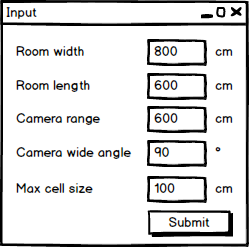
\includegraphics[scale=0.6]{input_mockup}
		\caption[Antarmuka penerima masukan]{Antarmuka penerima masukan}
		\label{fig:input_mockup}
	\end{figure}

	\item Antarmuka: \textbf{Simulasi Penempatan Kamera CCTV}\\
	Antarmuka ini berfungsi untuk melakukan kegiatan simulasi penempatan kamera CCTV. Antarmuka ini dapat dilihat pada gambar~\ref{fig:simulator_mockup}. Di dalam antarmuka ini terdapat 3 bagian, yaitu:
	\begin{itemize}
		\item Panel informasi yang berada di bagian kiri antarmuka.\\
		Panel ini berfungsi untuk memberikan informasi-informasi yang terdiri dari ukuran ruangan, spesifikasi kamera CCTV, informasi simulasi, dan daftar penempatan kamera CCTV. Pada bagian informasi simulasi terdapat informasi persentase ketercakupan dan persentase tingkat \textit{overlap} dan \textit{out of bound}. Pada bagian daftar penempatan kamera CCTV, terdapat penempatan-penempatan yang sedang diterapkan dalam simulasi. Pada setiap penempatan terdapat tombol ''\textit{remove}'' yang apabila ditekan akan membuang penempatan tersebut.
		
		\item Panel visualisasi penempatan kamera CCTV yang berada di bagian kanan antarmuka.\\
		Panel ini berfungsi untuk menampilkan visualisasi penempatan kamera CCTV sesuai dengan penempatan-penempatan yang sedang diterapkan pada simulasi.
		
		\item Panel penambah kamera CCTV yang berada di atas panel visualisasi.\\
		Panel ini berfungsi untuk melakukan penempatan kamera CCTV baru. Pengguna dapat melakukan 2 jenis penambahan penempatan, yaitu penambahan sesuai dengan keinginan pengguna dan penambahan secara otomatis. Apabila pengguna ingin melakukan penambahan sesuai dengan keinginan, maka pengguna dapat memilih posisi dan mengisi sudut arah pandang dan dilanjutkan dengan menekan tombol ''\textit{add camera}''. Apabila pengguna ingin melakukan penambahan secara otomatis, maka pengguna dapat menekan tombol ''\textit{auto place camera}''. Dengan melakukan penambahan secara otomatis, sistem akan mencari penempatan-penempatan tersedikit yang dapat mencakup seluruh cell yang belum tercakup. Selama proses penambahan otomatis berjalan, tombol ''\textit{add camera}'' dan tombol ''\textit{auto place camera}'' akan dinon-aktifkan dan diaktifkan kembali apabila proses telah selesai.
	\end{itemize}
	\begin{figure}[h]
		\centering  
		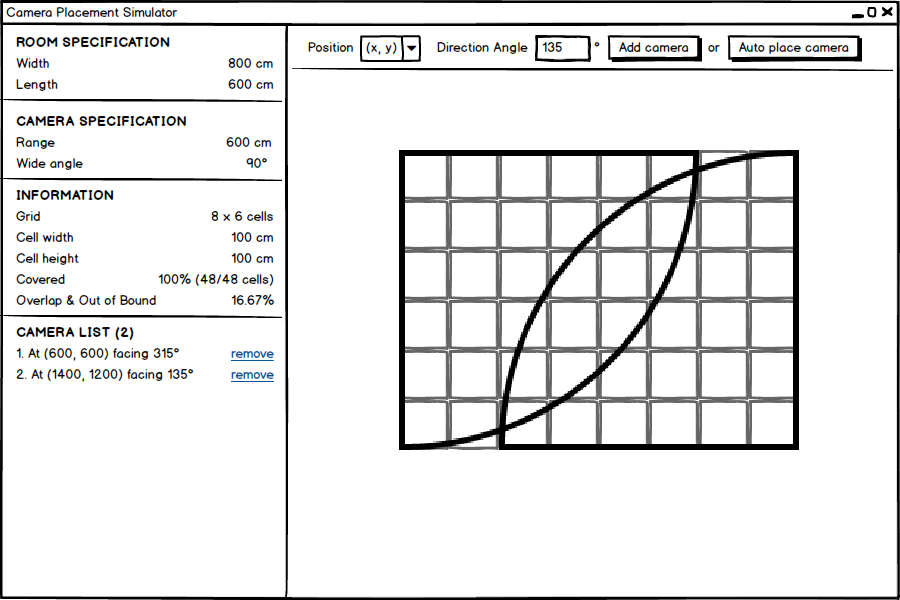
\includegraphics[scale=0.5]{simulator_mockup}
		\caption[Antarmuka penempatan kamera CCTV]{Antarmuka penempatan kamera CCTV}
		\label{fig:simulator_mockup}
	\end{figure}
\end{enumerate}

\section{Perancangan Kelas}
Pada bagian ini akan dijelaskan kelas-kelas yang digunakan dalam membangun perangkat lunak. Diagram kelas dapat dilihat pada gambar~\ref{fig:class_diagram_complete}.
\begin{sidewaysfigure}
	\centering  
	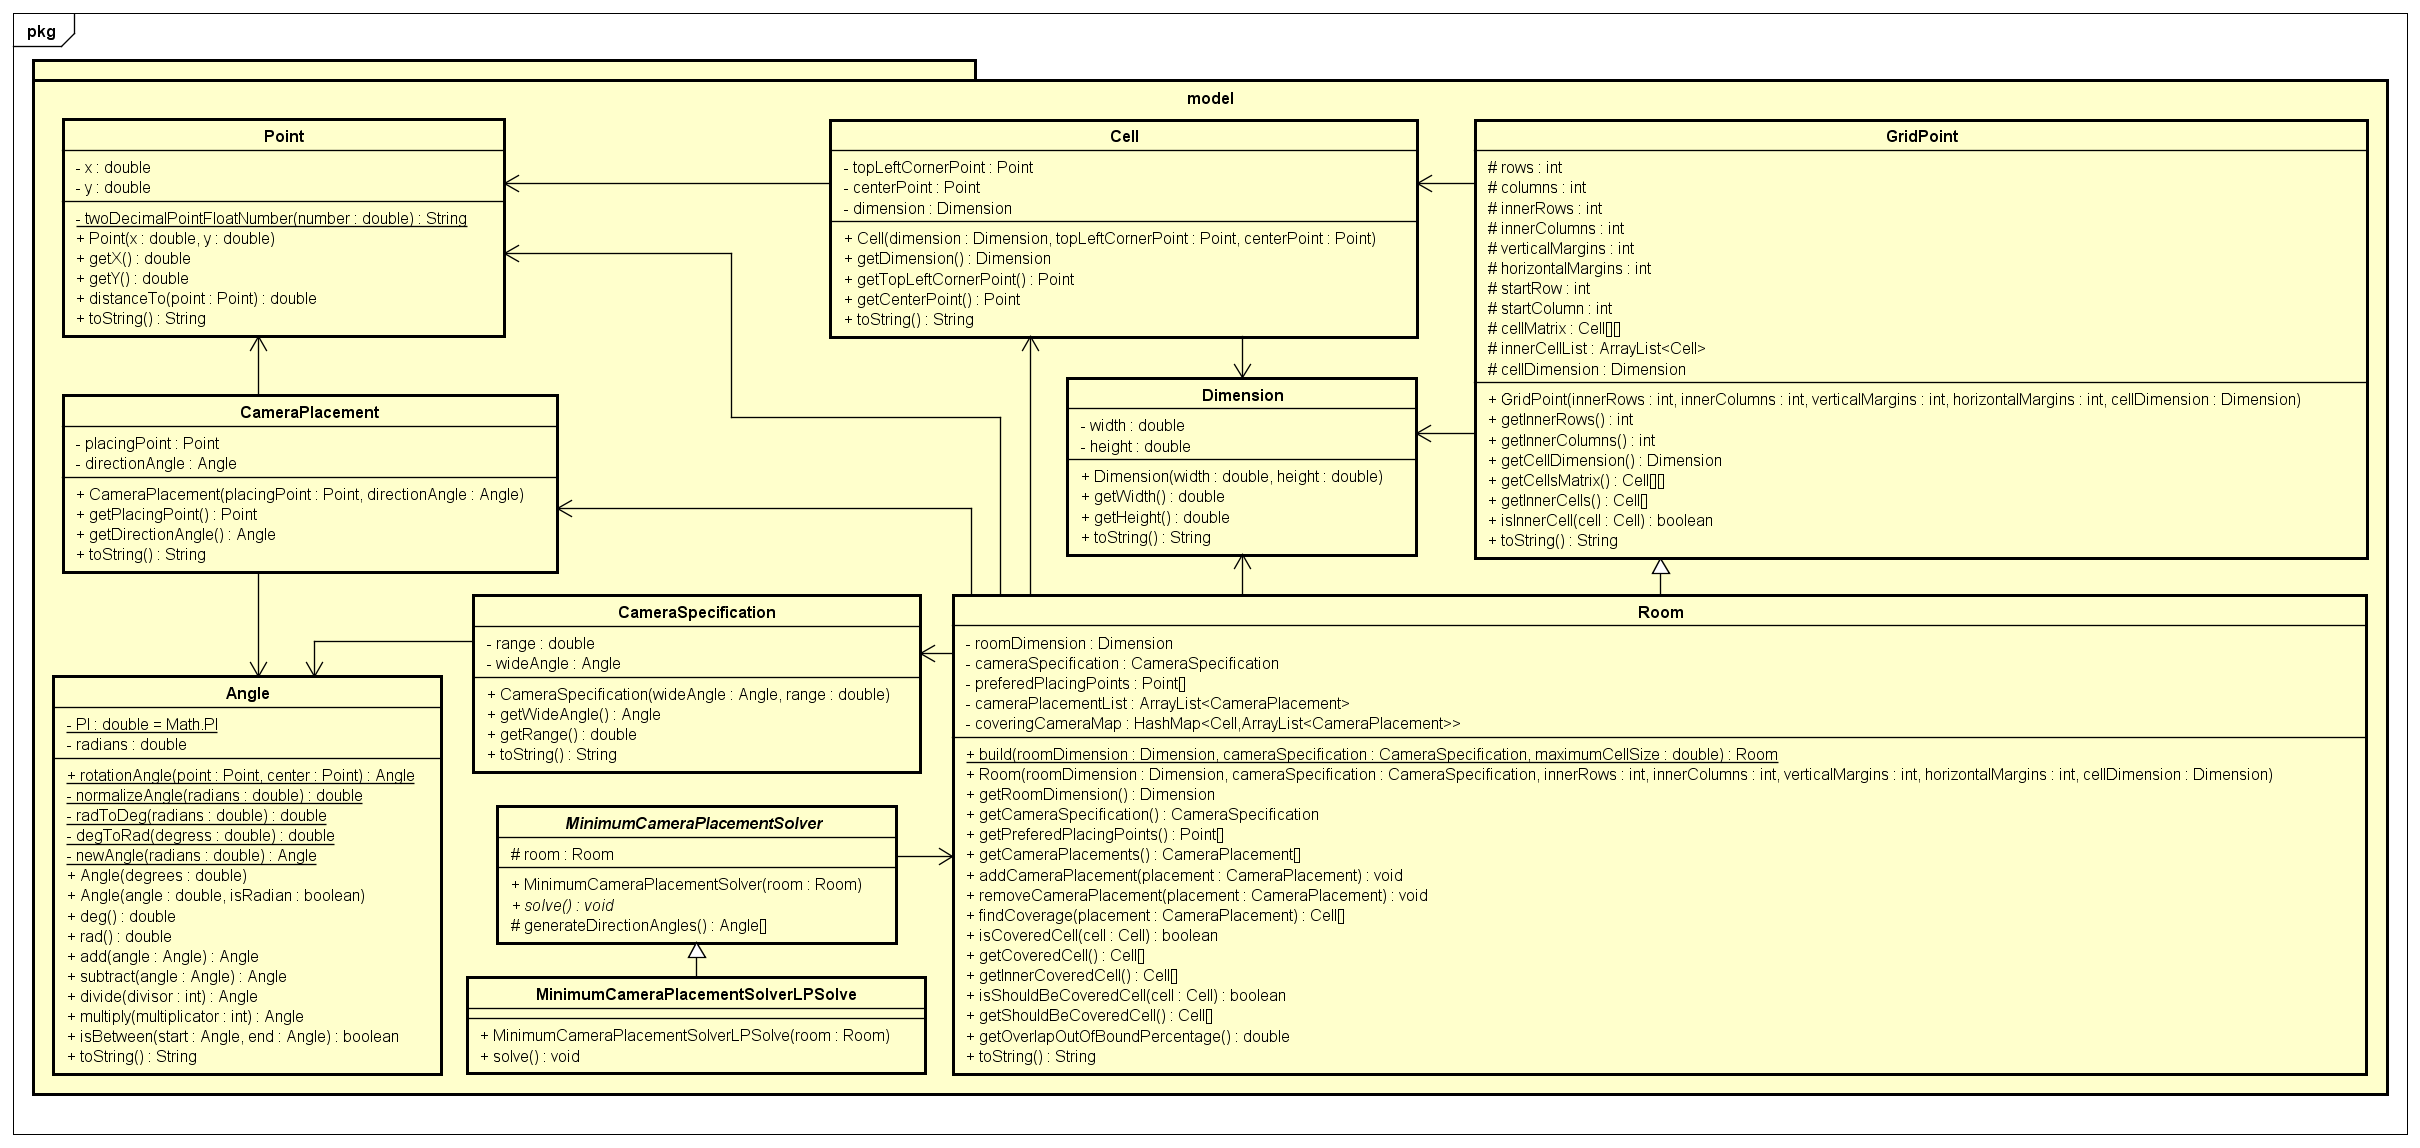
\includegraphics[scale=0.38]{class_diagram_complete}
	\caption[Kelas diagram]{Kelas diagram}
	\label{fig:class_diagram_complete}
\end{sidewaysfigure}

\subsection{Kelas \textit{Angle}}
\begin{figure}[H]
	\centering  
	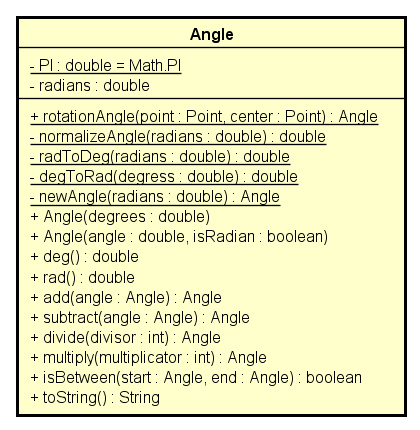
\includegraphics[scale=0.6]{class_angle}
	\caption[Diagram kelas \textit{Angle}]{Diagram kelas \textit{Angle}}
	\label{fig:class_angle}
\end{figure}
	
Kelas ini merepresentasikan sudut dan menangani fungsi-fungsi yang berhubungan dengan sudut. Diagram kelas \textit{Angle} dapat dilihat pada gambar~\ref{fig:class_angle}. Berikut ini merupakan atribut-atribut yang terdapat pada kelas \textit{Angle}:
\begin{itemize}
	\item \textbf{\textit{PI} \(\rightarrow\) \textit{double}}\\
	Atribut ini merupakan atribut statis bernilai \(\pi\) yang dapat digunakan oleh setiap objek dari kelas \textit{Angle}.
	\item \textbf{\textit{radians} \(\rightarrow\) \textit{double}}\\
	Atribut ini berguna untuk menampung sudut dalam bentuk radian.
\end{itemize}

Berikut ini merupakan fungsi-fungsi yang terdapat pada kelas \textit{Angle}:
\begin{itemize}
	\item \textbf{\textit{rotationAngle}(\textit{point} \(\rightarrow\) \textit{Point}, \textit{center} \(\rightarrow\) \textit{Point}) \(\rightarrow\) \textit{Angle}}\\
	Fungsi ini merupakan fungsi statis yang berguna untuk mendapatkan sudut rotasi dari titik \textit{point} terhadap titik \textit{center}.
	\item \textbf{\textit{normalizeAngle}(\textit{radians} \(\rightarrow\) \textit{double}) \(\rightarrow\) \textit{double}}\\
	Fungsi ini merupakan fungsi statis yang berguna untuk melakukan normalisasi sudut \textit{radians} sehingga berada dalam rentang \(0\leq\textit{radians}<2\pi\).
	\item \textbf{\textit{radToDeg}(\textit{radians} \(\rightarrow\) \textit{double}) \(\rightarrow\) \textit{double}}\\
	Fungsi ini merupakan fungsi statis yang berguna untuk mengubah sudut dalam bentuk radian menjadi sudut dalam bentuk derajat.
	\item \textbf{\textit{degToRad}(\textit{degrees} \(\rightarrow\) \textit{double}) \(\rightarrow\) \textit{double}}\\
	Fungsi ini merupakan fungsi statis yang berguna untuk mengubah sudut dalam bentuk derajat menjadi sudut dalam bentuk radian.
	\item \textbf{\textit{newAngle}(\textit{radians} \(\rightarrow\) \textit{double}) \(\rightarrow\) \textit{Angle}}\\
	Fungsi ini merupakan fungsi statis yang berguna untuk membuat instansiasi baru dari kelas \textit{Angle}.
	\item \textbf{\textit{deg}() \(\rightarrow\) \textit{double}}\\
	Fungsi ini berguna untuk mendapatkan sudut dalam bentuk derajat.
	\item \textbf{\textit{rad}() \(\rightarrow\) \textit{double}}\\
	Fungsi ini berguna untuk mendapatkan sudut dalam bentuk radian.
	\item \textbf{\textit{add}(\textit{angle} \(\rightarrow\) \textit{Angle}) \(\rightarrow\) \textit{Angle}}\\
	Fungsi ini berguna untuk menghasilkan objek sudut baru yang merupakan hasil penjumlahan antara sudut objek ini dengan sudut objek \textit{angle}.
	\item \textbf{\textit{subtract}(\textit{angle} \(\rightarrow\) \textit{Angle}) \(\rightarrow\) \textit{Angle}}\\
	Fungsi ini berguna untuk menghasilkan objek sudut baru yang merupakan hasil pengurangan antara sudut objek ini dengan sudut objek \textit{angle}.
	\item \textbf{\textit{divide}(\textit{divisor} \(\rightarrow\) \textit{int}) \(\rightarrow\) \textit{Angle}}\\
	Fungsi ini berguna untuk menghasilkan objek sudut baru yang merupakan hasil pembagian antara sudut objek ini dengan nilai \textit{divisor}.
	\item \textbf{\textit{multiply}(\textit{multiplicator} \(\rightarrow\) \textit{int}) \(\rightarrow\) \textit{Angle}}\\
	Fungsi ini berguna untuk menghasilkan objek sudut baru yang merupakan hasil pengalian antara sudut objek ini dengan nilai \textit{multiplicator}.
	\item \textbf{\textit{isBetween}(\textit{start} \(\rightarrow\) \textit{Angle}, \textit{end} \(\rightarrow\) \textit{Angle}) \(\rightarrow\) \textit{boolean}}\\
	Fungsi ini berguna untuk mengetahui apakah sudut objek ini berada di antara sudut objek \textit{start} dan sudut objek \textit{end}.
\end{itemize}

\subsection{Kelas \textit{Point}}
\begin{figure}[H]
	\centering  
	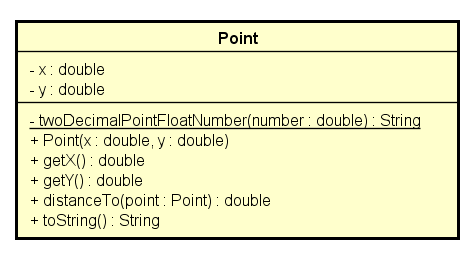
\includegraphics[scale=0.6]{class_point}
	\caption[Diagram kelas \textit{Point}]{Diagram kelas \textit{Point}}
	\label{fig:class_point}
\end{figure}

Kelas ini merepresentasikan titik koordinat 2D. Diagram kelas \textit{Point} dapat dilihat pada gambar~\ref{fig:class_point}. Berikut ini merupakan atribut-atribut yang terdapat pada kelas \textit{Point}:
\begin{itemize}
	\item \textbf{\textit{x} \(\rightarrow\) \textit{double}}\\
	Atribut ini berguna untuk menampung nilai titik pada sumbu x.
	\item \textbf{\textit{y} \(\rightarrow\) \textit{double}}\\
	Atribut ini berguna untuk menampung nilai titik pada sumbu y.
\end{itemize}

Berikut ini merupakan fungsi-fungsi yang terdapat pada kelas \textit{Point}:
\begin{itemize}
	\item \textbf{\textit{twoDecimalPointFloatNumber}(\textit{number} \(\rightarrow\) \textit{double}) \(\rightarrow\) \textit{String}}\\
	Fungsi ini merupakan fungsi statis yang berguna untuk mengubah bilangan \textit{number} ke dalam bentuk \textit{String} dengan maksimal bilangan di belakang koma berjumlah 2 buah.
	\item \textbf{\textit{distanceTo}(\textit{point} \(\rightarrow\) \textit{Point}) \(\rightarrow\) \textit{double}}\\
	Fungsi ini berguna untuk mendapatkan jarak antara titik objek ini dengan titik objek \textit{point}.
\end{itemize}



























